\documentclass[titlepage]{report}

\usepackage{titlesec}
\usepackage{lipsum}
\usepackage{graphicx}
\usepackage{wrapfig}

%setting for chapter font
\titleformat{\chapter}[display]
  {\Huge\bfseries}{}{1pt}{\Huge}
  
  
\author{ALL Author Names}
\title{\textbf{CustoNN2: Customizing Neural Networks on FPGAs}}  
  
  
\begin{document}

\maketitle

\tableofcontents
\newpage

\chapter{Introduction}
In recent times Convolutional Neural Networks (CNN) has gained immense popularity and is used in many applications such as Image classification , speech recognition etc. CNNs have become an industry standard and provide a near human accuracy. However CNN are computationally intensive models requiring large amount of processing power which calls for the need to have dedicated hardware for its acceleration. Graphics Processing Units (GPU) are conventionally used and provide satisfactory performance on some of the state-of-the-art CNN models. Although GPU provides good performance, its not flexible enough to accomodate multiple CNN models. One may need to re-design the entire GPU architecture for a particular CNN. This is where Field Programmable Gate Arrays (FPGA) proves to be much more beneficial in terms of flexibility and parallel processing. Some state-of the-art CNN models such as AlexNet , VGG16 and ResNet has shown considerable performance gain using FPGAs. Futhermore with the presence of various Software Development (SDK) Toolkit in the market such as Intel OpenVINO, Xilinx ML Suite and TVM has helped the developers to efficiently map their CNN models to the underlying architecture. Due to all of these factors CNN has become a popular choice for image classification applications.


\section{Why FPGA}
There are multiple hardware avaliable in the market such as CPU, GPU , ASIC and FPGA each used for a specific set of application. Among all of them FPGAs are becoming widely poplular and used in CNN based applications. Deep Neural Networks (DNN) benefit very much from using FPGA. DNN are math intensive models which execute the same or many mathematical operation. FPGAs have dedicated DSPs and ALUs to perform such Floating Point arithmetic operations. FPGAs are suited for applications which uses custom datatypes which is the case in DNN. Also they provide better latency, parallel processing power and flexibility among all its counterparts. Using FPGA also has another specific advantage. The advantage is that it can accomodate different CNN models without the need of changing the underlying architecture. CNN models have a streaming architecture that suits well with FPGA architecture.
In this project we are using the Intel Stratix 10 F1760 NF43 package with 520N Scalable FPGA Network Accelerator Card for our CNN inference on Image classification . Paderborn Center for Parallel Computing (PC2) has 32 of this FPGA and our task is to scale our CNN architecture using all 32 FPGAs. We will be using three pre-trained model namely GoogleNet, ResNet-52 and Inception V4 in a model ensemble architecture where majority voting is used. The workload will be divided among all the 32 FPGAs and the layers will be distributed to each of these FPGAs in a streaming architecture fashion. Atlast we will measure the performance of our system using some performance metrics.

% Remove below lipsum command before posting your work
\lipsum[3]

\section{CNNs}

% Remove below lipsum command before posting your work
\lipsum[3]


%End of the chapter

\chapter{Goals}

\section{Scaling over multiple FPGAs}

% Remove below lipsum command before posting your work
\lipsum[3]

\section{Performance Optimization}
% Remove below lipsum command before posting your work
\lipsum[3]

\section{Quantization / Pruning}
% Remove below lipsum command before posting your work
\lipsum[3]


%End of the chapter

\chapter{Topologies, datasets. Architecture comparision}

\section{Topologies}
% Remove below lipsum command before posting your work
\lipsum[3]

\subsection{Inception v4}
Inception-V4 is a deep neural network (DNN) released by Google. Inception-V4 is a fourth version of inception module and includes all techniques from Inception-V1, Inception-V2, and Inception-V3. Google devised inception module and it was a key idea for Inception-V1. The naïve version of the first inception module included 1×1, 3×3 and 5×5 convs and max-pooling as input and the result of concatenated them together as output. \\
\pagebreak
\begin{wrapfigure}{l}{0.5\textwidth}
\centering
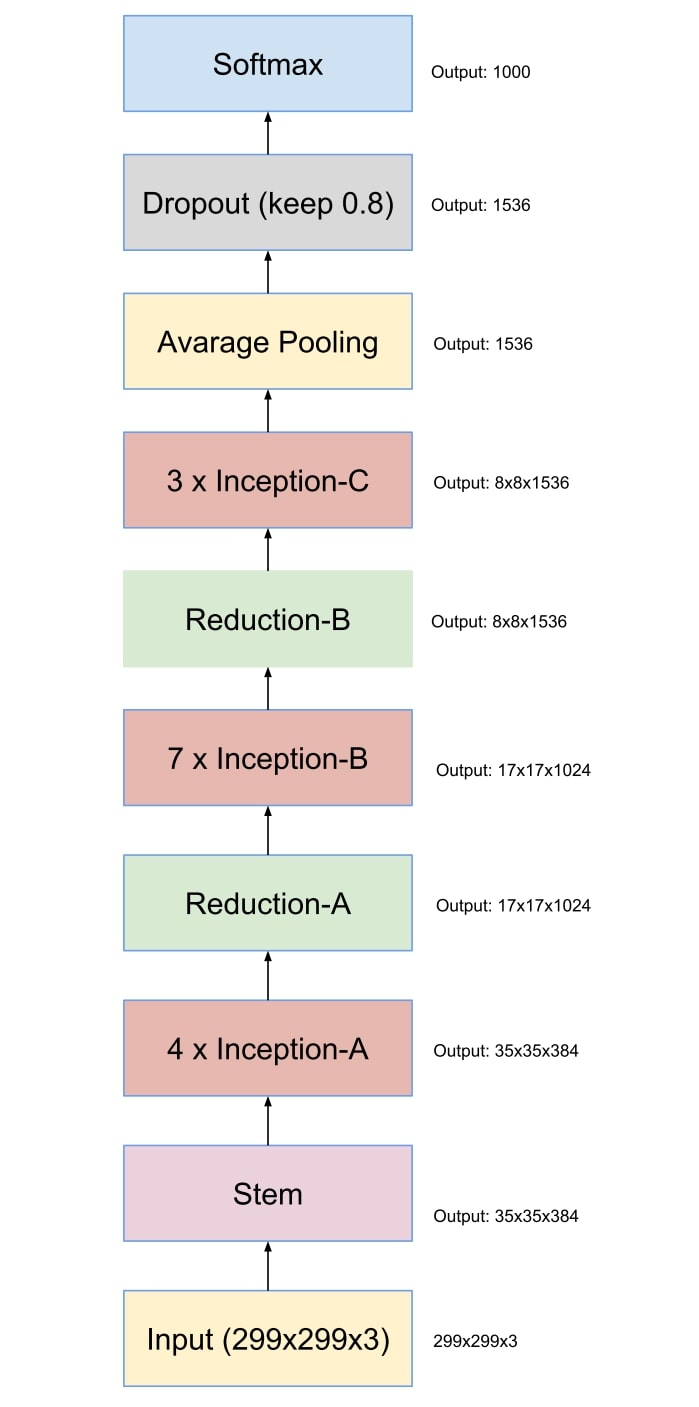
\includegraphics[scale=0.3]{inception_v4}
\caption{Inception-V4}
\label{fig:inception_v4}
\end{wrapfigure}

The contribution from Inception-V2 is batch normalization. They use ReLU as activation function in order to avoid the saturation problem and vanishing gradients. They had to use a higher learning rate for regularization because the output became more irregular. Last changes was reducing dimension by replacing   5×5 conv to two 3×3 convs. 

Inception-V4 also used the factorization from the Inception-V3. They reduce the dimensionality and it helped to decrease the overfitting problem. For example, if you have a 3×3 filter then you need 9 parameters, but the factorization idea proposes to operate  3×1 and  1×3 filters and use only 6 parameters. 

Inception-V4 have 3.1\% in Top-5 error rate and this result is better than winner of 2015 year ResNet (3.57\%) and  Inception-V3 (3.58\%). 

Inception architecture has a relatively low computation cost. Google try to make the inception module more efficient that's why they made it deeper and wider then Inception-V3 and they also simplify the architecture of this DNN.

Figure \ref{fig:inception_v4} shows the whole scheme for Inception-V4.

\subsection{GoogleNet}
% Remove below lipsum command before posting your work
\lipsum[3]

\subsection{Resnet50}
ResNet is another deep neural network released by Microsoft and, also, a winner of ILSVRG 2015 in image classification, detection, and localization. ResNet is a series of DNN with different numbers of layers from 18 to 152. The base idea is applying the residual connections which are described as learning the residual representation of functions instead of signal representation. One of the conceptual ideas of ResNet is using the skip connection. Skip connection makes the network deeper.  

Many convolution DNNs run into a problem with vanishing or exploding gradients because, during backpropagation, we derive error function with respect to the current weight and get multiplying of small or large numbers. The product of small numbers will be zero (vanished) and the product of large numbers will be too large (exploded). Developers of ResNet solved this problem by using a skip connection. In the skip connections for the next layer, they use the input from the previous layer without any modification. 

\begin{figure}[h!]
    \centering
    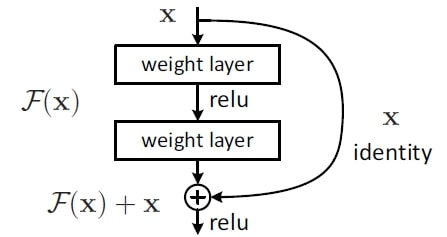
\includegraphics[scale=0.4]{resnet_1}
    \caption{Skip connection}
\end{figure}

\begin{wrapfigure}{l}{0.5\textwidth}
\centering
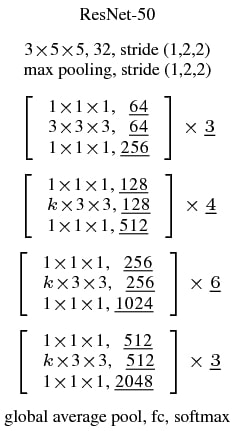
\includegraphics[scale=0.8]{resnet_2}
\caption{ResNet-50}
\label{fig:resnet_50}
\end{wrapfigure}

The output of skip connection is  F(x) + x and the weight layers actually are to learn a kind of residual mapping: output minus identity x. If we have a vanishing gradient we always have an identity x to send it back to previous layers. 

After each convolution layer ResNet use the batch normalization from Inception-V2. 

The main concepts of construction ResNet:
\begin{itemize}
  \item avoiding representational bottlenecks by not abruptly reduce the dimension of data,but smoothly from the beginning of the network to the classifier at the output;
  \item factorization of convolution layer into smaller pieces because this will save resources and help to increase the count of layers;
  \item supporting a balance between the depth and width of the network. You should increase or decrease both dimensions.
\end{itemize}

Figure \ref{fig:resnet_50} shows the whole scheme for ResNet-50.


\section{Datasets}
% Remove below lipsum command before posting your work
\lipsum[3]

\subsection{Imagenet}
% Remove below lipsum command before posting your work
\lipsum[3]

\subsection{CIFAR10}
% Remove below lipsum command before posting your work
\lipsum[3]

\subsection{MNIST}
% Remove below lipsum command before posting your work
\lipsum[3]

%End of the chapter



\chapter{Metrics}

\section{FLOPS using performance modelling}
% Remove below lipsum command before posting your work
\lipsum[3]

\section{Latency, Throughput}
% Remove below lipsum command before posting your work
\lipsum[3]

\section{Accuracy}
% Remove below lipsum command before posting your work
\lipsum[3]


%End of the chapter


\chapter{Flowcharts}
% Remove below lipsum command before posting your work
\lipsum[3]


%End of the chapter

\chapter{Technologies}

\section{OpenVINO}
% Remove below lipsum command before posting your work
Intel OPENVINO is an open source toolkit from Intel that allows the deployment of pre-trained deep neural networks on different hardware platforms such as CPU, GPU, FPGA etc. The toolkit is available for installation for the Windows operating system as well as selected Linux distributions. All of the tool's libraries and plugins except the FPGA plugin are a part of the open source github repository.
The functionality of OPENVINO is divided among its components, Model Optimizer and Inference Engine.

\subsection{Model Optimizer}
The Model Optimizer is a python based tool which takes as input a pre-trained model. It supports many popular deep learning frameworks such as TensorFlow, Caffe, PyTorch, MXnet etc. This model is then converted to a common intermediate format (IR), thereby making the inference engine independent of the training framework. The IR contains a .xml file which represents the computational graph of the CNN and a .bin file containing the weights. The graph is optimized by fusing different layers of the original topology wherever possible. The weights are accordingly adjusted. 
 
 \subsection{Inference Engine}
 The Inference Engine is responsible for the execution of the model on the selected hardware. For this purpose, it provides a C++ API which can be integrated in an application. The main task performed by the inference engine is to read the Intermediate Representation of the model, select the hardware for deployment such as CPU or FPGA and call the appropriate plugin which defines all necessary data structures and functions required to perform inference and return the output along with performance statistics. 
 The toolkit comes with pre-compiled bitstreams (.aocx files) for a few supported FPGA boards. These bitstreams implement various popular network topologies such as GoogleNet, ResNet etc. as well as generic layers which are used to program the FPGAs as per the requirement of the given model topology. 
 
 \subsection{Advantages and Disadvantages}
  
 \begin{itemize}
 \item Supports optimization of models and quantization of weights.
 \item A CNN model can be deployed on hardware with minimal programming effort and independent of the training framework.
 \item For FPGAs, the use of pre-compiled bitstreams eliminate the time needed for synthesis of kernel codes.
 \item The only disadvantage is the compatibility of FPGA boards. Development and synthesis of kernel codes along with a plugin for FPGAs may be required to make OPENVINO work with unsupported boards. 
 
 \end{itemize}

\section{TVM}
% Remove below lipsum command before posting your work
\lipsum[3]

\section{Xilinx}
% Remove below lipsum command before posting your work
\lipsum[3]

%End of the chapter

\chapter{Related Work}
% Remove below lipsum command before posting your work
\lipsum[3]


%End of the chapter

\chapter{Time plan}

\section{Design}
% Remove below lipsum command before posting your work
\lipsum[3]

\section{Implementation}
% Remove below lipsum command before posting your work
\lipsum[3]

\section{Report and Presentation}
% Remove below lipsum command before posting your work
\lipsum[3]

\section{Organization}
% Remove below lipsum command before posting your work
\lipsum[3]

%End of the chapter


\chapter{Expected Results}
% Remove below lipsum command before posting your work
\lipsum[3]

\section{Final OutPuts}

% Remove below lipsum command before posting your work
\lipsum[3]

%End of the chapter

\chapter{Conclusion}

% Remove below lipsum command before posting your work
\lipsum[2]

%End of the chapter

\end{document}
